%% =============================================================================
%% chapters/appendix-infrastructure-configuration.tex
%% Appendix H: Platform Infrastructure, MicroK8s & Middleware Configuration Specification
%% =============================================================================

\chapter{Platform Infrastructure, MicroK8s \& Middleware Configuration}
\label{app:infrastructure_configuration}
{\textit{\textbf{Authoritative Platform Specification, MicroK8s Add-on Architecture, Declarative Middleconfiguration, Middleware Parameters, and Operational Automation Runbooks}}}

\section{Platform Overview \& Infrastructure Separation Strategy}
\label{sec:infra_overview}

The \textbf{Harmonia Health Information Exchange (HIE)} platform is designed to operate seamlessly across bare-metal servers, virtualized instances, and enterprise cloud infrastructure. To achieve high operational predictability, rapid fault isolation, and reproducible deployments with zero configuration drift, Harmonia enforces a strict five-stage architectural separation of concerns between runtime application logic and infrastructure orchestration:

\begin{figure}
	\setlength{\fboxrule}{0.5pt}
	\setlength{\fboxsep}{3pt}
	\centering
	\fbox{%
        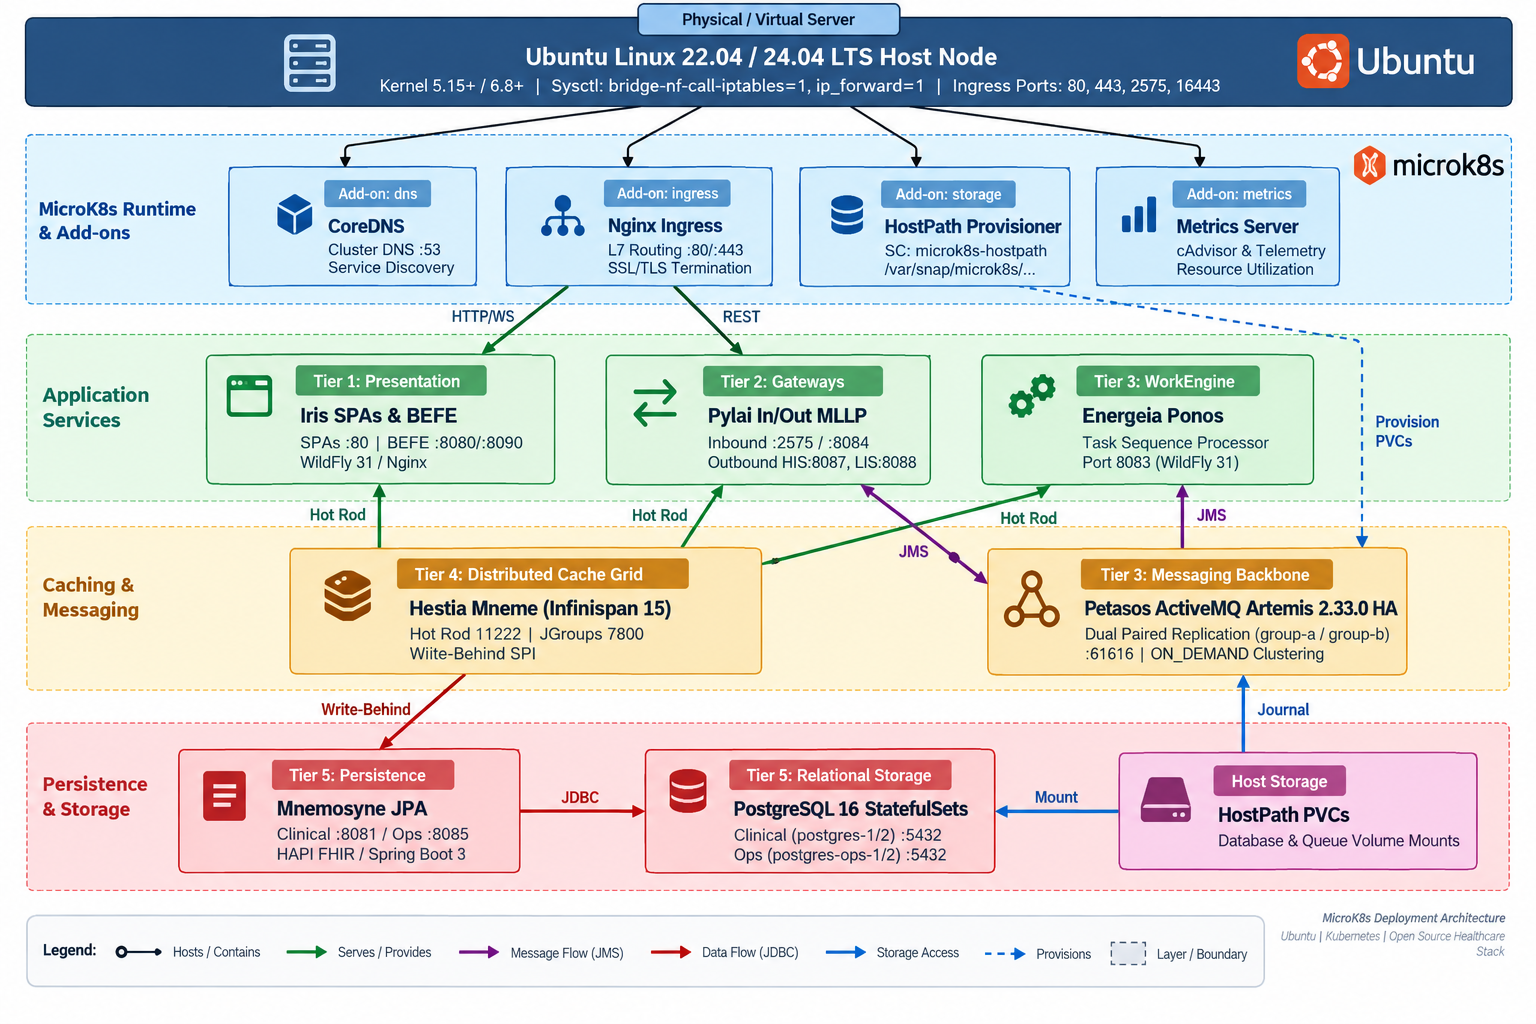
\includegraphics[width=0.94\textwidth, height=0.82\textheight,keepaspectratio]
        {images/physical-infrastructure-microk8s-add-ons-and-5-tier-workload-deployment-topology.png}
    }
    \caption{ArchiMate 3.2 Physical Infrastructure, MicroK8s Add-ons, and 5-Tier Workload Deployment Topology}
    \label{fig:microk8s_infrastructure}
\end{figure}

\subsection{Architectural Separation of Concerns}

The separation model guarantees that software artifacts remain completely environment-agnostic while enabling automated provisioning across development, testing, staging, and production environments:

\begin{enumerate}[label=\textbf{\arabic*.}]
    \item \textbf{Harmonia Application Logic (Java 21 / Spring Boot 3 / WildFly 31 / Vue 3)}: All business logic, FHIR resource modeling, transactional state machines, and cryptographic authorization routines are contained in upstream source modules. Code contains zero hardcoded hostnames, distribution-specific hooks, or environment-conditional branching (e.g. \texttt{if (microk8s)}).
    \item \textbf{OCI Container Images}: Standard Open Container Initiative (OCI) images are packaged using Maven container profiles (\texttt{-Pcontainer-build}, \texttt{-Pcontainer-publish}) with standardized entrypoints, unprivileged service execution accounts, and parameterization via POSIX environment variables.
    \item \textbf{Authoritative Kubernetes Manifests (Kustomize Base)}: Located in \texttt{deployment/kubernetes/base/}, these declarative YAML resources define the cluster blueprint: Deployments, StatefulSets, ClusterIP Services, Ingress objects, NetworkPolicies, and PersistentVolumeClaims.
    \item \textbf{Environment Overlays (MicroK8s / Multi-Node)}: Located in \texttt{deployment/kubernetes/environments/}, declarative Kustomize overlays apply environment-specific patches (such as the \texttt{microk8s-hostpath} storage class or node port assignments) without modifying base manifests.
    \item \textbf{Ansible Automation Engine}: Located in \texttt{deployment/ansible/}, automated playbooks orchestrate host-level sysctl kernel tuning, snap package lifecycle, add-on activation, secret injection from encrypted vaults, and rollout verification loops.
\end{enumerate}

\begin{principlebox}{1. Declarative Infrastructure as Code (IaC) Invariant}
No deployment, configuration change, or volume binding may be executed manually via ad-hoc terminal interventions. All cluster state must originate from declarative Kustomize manifests and Ansible playbooks under strict Git version control.
\end{principlebox}

\subsection{Single-Node MicroK8s Resilience Semantics vs Multi-Node Scaling}

Harmonia designates single-node \textbf{MicroK8s on Ubuntu Linux} as its authoritative baseline deployment target. In this topology:
\begin{itemize}
    \item \textbf{Pod \& Process Restart Resilience}: The Kubernetes kubelet and containerd runtime automatically recover crashed application containers, microservices, and database processes with sub-second restart loops.
    \item \textbf{State Persistence across Node Reboots}: StatefulSets (Artemis messaging journals, PostgreSQL database tables, and Infinispan cache partitions) mount persistent volumes through the local \texttt{microk8s-hostpath} provisioner, preserving transactional integrity across operating system restarts.
    \item \textbf{Zero-Friction Multi-Node Evolution}: Because manifests in \texttt{deployment/kubernetes/base/} use standard Kubernetes API primitives, transitioning to multi-node clusters requires only substituting the \texttt{microk8s-hostpath} StorageClass with a CSI network provisioner (e.g. Ceph RBD, AWS EBS, NFS) and adding \texttt{podAntiAffinity} scheduling constraints.
\end{itemize}

% =============================================================================
% SECTION H.2: PLATFORM & HOST INFRASTRUCTURE PREREQUISITES
% =============================================================================
\section{Platform \& Host Infrastructure Prerequisites}
\label{sec:host_prerequisites}

\subsection{Supported Operating Systems \& Architecture Support}

Harmonia is tested and certified on canonical enterprise Linux distributions:
\begin{itemize}
    \item \textbf{Ubuntu Linux 22.04 LTS (Jammy Jellyfish)}: 64-bit x86 (\texttt{x86\_64} / \texttt{amd64}) and 64-bit ARM (\texttt{aarch64} / \texttt{arm64}).
    \item \textbf{Ubuntu Linux 24.04 LTS (Noble Numbat)}: 64-bit x86 (\texttt{x86\_64} / \texttt{amd64}) and 64-bit ARM (\texttt{aarch64} / \texttt{arm64}).
\end{itemize}

Automated host initialization via \texttt{deployment/ansible/roles/microk8s/tasks/prerequisites.yml} ensures the installation of core system utilities: \texttt{snapd}, \texttt{iptables}, \texttt{curl}, \texttt{conntrack}, \texttt{socat}, and \texttt{ca-certificates}.

\subsection{Hardware Sizing Profiles \& Resource Allocation Matrix}

Harmonia provides three standardized sizing profiles calibrated for varying computational demands:

\begin{table}[htbp]
\centering
\small
\begin{tabularx}{\textwidth}{l C{2.0cm} C{2.2cm} C{2.6cm} X}
\toprule
\textbf{Sizing Profile} & \textbf{vCPU Cores} & \textbf{RAM} & \textbf{Storage (SSD/NVMe)} & \textbf{Operational Scope \& Use Case} \\
\midrule
\textbf{Minimum Reference} & 4 vCPU & 8 GB & 40 GB & \textbf{CI/CD \& Functional Verification}: Single-node functional smoke testing, integration test pipelines, and developer environments. \\
\addlinespace
\textbf{Recommended Dev/Test} & 8 vCPU & 16 GB & 100 GB & \textbf{Integration \& Load Simulation}: End-to-end multi-module testing, MLLP message simulation, and cache clustering verification. \\
\addlinespace
\textbf{Production Target} & 16+ vCPU & 32+ GB & 250+ GB (Fast NVMe) & \textbf{High-Throughput Clinical HIE}: Sustained HL7/FHIR ingest streams, dual Artemis HA journal replication, and write-behind persistence bursts. \\
\bottomrule
\end{tabularx}
\caption{Harmonia Host Platform Sizing Profiles and Resource Allocation Matrix}
\label{tab:hardware_sizing}
\end{table}

\subsection{Linux Kernel Networking \& Sysctl Configuration}

Kubernetes container networking and high-volume clinical messaging require specific Linux kernel parameters to prevent packet drops, connection tracking exhaustion, and file descriptor starvation:

\begin{table}[htbp]
\centering
\small
\begin{tabularx}{\textwidth}{l c p{4.2cm} X}
\toprule
\textbf{Kernel Parameter (\texttt{sysctl})} & \textbf{Value} & \textbf{Subsystem Impact} & \textbf{Technical Justification} \\
\midrule
\texttt{net.bridge.bridge-nf-call-iptables} & \texttt{1} & Bridge Netfilter & Forces bridged IPv4 traffic through host \texttt{iptables} chains for Kubernetes CNI packet filtering. \\
\addlinespace
\texttt{net.bridge.bridge-nf-call-ip6tables} & \texttt{1} & Bridge Netfilter IPv6 & Forces bridged IPv6 packets through \texttt{ip6tables} filtering rules. \\
\addlinespace
\texttt{net.ipv4.ip\_forward} & \texttt{1} & IPv4 Forwarding & Enables IP packet forwarding between the physical host network adapter and virtual CNI pod network interfaces. \\
\addlinespace
\texttt{fs.inotify.max\_user\_watches} & \texttt{524288} & Inotify Subsystem & Prevents filesystem event watcher exhaustion across containerized WildFly deployments and Hot Rod log listeners. \\
\addlinespace
\texttt{vm.max\_map\_count} & \texttt{262144} & Virtual Memory Mappings & Ensures sufficient memory map areas for Infinispan 15 data grid off-heap memory allocations and JVM thread stacks. \\
\addlinespace
\texttt{vm.swappiness} & \texttt{10} & Memory Swapping Policy & Minimizes aggressive swap activity to preserve deterministic low latency across Petasos Artemis and Mneme cache nodes. \\
\bottomrule
\end{tabularx}
\caption{Authoritative Linux Kernel Parameters and Sysctl Network Tuning}
\label{tab:sysctl_parameters}
\end{table}

\subsection{Host Firewall, Ingress Routing \& Port Exposure Matrix}

Table~\ref{tab:firewall_ports} defines the network ingress and inter-service port allocations that must be open on the host operating system firewall (e.g. \texttt{ufw} or cloud security groups).

\begin{table}[htbp]
\centering
\small
\begin{tabularx}{\textwidth}{l c l X}
\toprule
\textbf{Port / Protocol} & \textbf{Exposure} & \textbf{Target Component} & \textbf{Functional Description} \\
\midrule
\texttt{80/tcp} & External & Nginx Ingress & Plaintext HTTP ingress routing for Iris SPAs and BEFE APIs. \\
\texttt{443/tcp} & External & Nginx Ingress & TLS-terminated HTTPS ingress for production browser interfaces. \\
\texttt{2575/tcp} & External & Pylai Inbound MLLP & Minimal Lower Layer Protocol (MLLP) clinical HL7 v2 ingest gateway. \\
\texttt{16443/tcp} & Bastion/LAN & MicroK8s Kube-API & MicroK8s Kubernetes control plane API server for \texttt{kubectl} and Ansible. \\
\addlinespace
\texttt{10.1.0.0/16} & Cluster Internal & Calico / Host CNI & Internal Pod network overlay CIDR for inter-pod routing. \\
\texttt{10.152.183.0/24} & Cluster Internal & Kube-Proxy / Services & Internal ClusterIP service virtual IP network range. \\
\bottomrule
\end{tabularx}
\caption{Host Network Port Matrix and Firewall Exposure Rules}
\label{tab:firewall_ports}
\end{table}

% =============================================================================
% SECTION H.3: MICROK8S COMPONENT ARCHITECTURE & ADD-ONS
% =============================================================================
\section{MicroK8s Component Architecture \& Add-on Specification}
\label{sec:microk8s_addons}

\subsection{Snap Packaging, Confinement \& Permission Management}

MicroK8s is deployed via Canonical's \texttt{snapd} package manager using classic confinement:
\begin{itemize}
    \item \textbf{Snap Channels}: Harmonia supports the \texttt{1.28/stable} baseline channel (configured in \texttt{deployment/ansible/roles/microk8s/defaults/main.yml}) and \texttt{1.30/stable} target channel.
    \item \textbf{Classic Confinement (\texttt{--classic})}: Grants MicroK8s full access to host storage devices, network interfaces, and kernel cgroups necessary for unhindered container orchestration.
    \item \textbf{Group Permissions}: The operational user (default \texttt{ubuntu}) is assigned to the \texttt{microk8s} POSIX group, granting unprivileged access to the \texttt{microk8s} CLI without requiring \texttt{sudo} elevation.
    \item \textbf{Kubeconfig Synchronization}: The playbook automatically initializes \texttt{\textasciitilde/.kube/config} with client certificates extracted from \texttt{/var/snap/microk8s/current/credentials/client.config}.
\end{itemize}

\subsection{Authoritative Add-on Matrix}

Harmonia requires four fundamental MicroK8s add-ons, systematically validated and activated by \texttt{deployment/ansible/roles/microk8s/tasks/addons.yml}:

\begin{table}[htbp]
\centering
\small
\begin{tabularx}{\textwidth}{l p{2.8cm} p{3.2cm} X}
\toprule
\textbf{Add-on Name} & \textbf{Underlying Technology} & \textbf{Cluster Address / Target} & \textbf{Role \& Platform Justification} \\
\midrule
\texttt{dns} & CoreDNS 1.10+ & \texttt{10.152.183.10:53} (UDP/TCP) & Provides dynamic, resilient service discovery for internal microservice resolution (e.g. \texttt{infinispan-1.harmonia.svc.cluster.local}). \\
\addlinespace
\texttt{ingress} & Ingress-Nginx 1.9+ & Host Ports \texttt{80/tcp}, \texttt{443/tcp} & Delivers centralized Layer 7 ingress routing, proxy buffer management, and SSL/TLS termination for SPAs and REST endpoints. \\
\addlinespace
\texttt{hostpath-storage} & Dynamic HostPath Provisioner & \texttt{/var/snap/microk8s/common/default-storage/} & Satisfies PersistentVolumeClaims (PVCs) by provisioning dedicated local host directories under StorageClass \texttt{microk8s-hostpath}. \\
\addlinespace
\texttt{metrics-server} & Kubernetes Metrics Server & Kubelet cAdvisor Telemetry & Exposes real-time CPU and memory utilization metrics to \texttt{kubectl top} and automated deployment verification gates. \\
\bottomrule
\end{tabularx}
\caption{Authoritative MicroK8s Add-on Specification and Capabilities}
\label{tab:microk8s_addons}
\end{table}

\subsection{CoreDNS Add-on (\texttt{dns}) Configuration}

CoreDNS runs as a cluster-internal deployment in the \texttt{kube-system} namespace. It provides authoritative DNS resolution for the \texttt{cluster.local} domain while forwarding unhandled upstream domain lookups to the host system's resolver defined in \texttt{/etc/resolv.conf}.

\begin{lstlisting}[language=XML, caption={CoreDNS Upstream Forwarding and Service Resolution Scheme}, label={lst:coredns_config}]
# Internal Resolution Examples:
infinispan-1.harmonia.svc.cluster.local       -> 10.152.183.42:11222
postgres-1.harmonia.svc.cluster.local         -> 10.152.183.88:5432
task-processor.harmonia.svc.cluster.local     -> 10.152.183.95:61616
befe.harmonia.svc.cluster.local               -> 10.152.183.110:8080
\end{lstlisting}

\subsection{Nginx Ingress Controller (\texttt{ingress}) Specification}

The Nginx Ingress Controller routes external traffic to the 5-tier workloads. Harmonia's base ingress resource (\texttt{deployment/kubernetes/base/ingress.yaml}) configures specific proxy buffer and timeout annotations to accommodate clinical throughput:

\begin{lstlisting}[language=XML, caption={Ingress Annotations and Host Routing Rules}, label={lst:ingress_yaml}]
apiVersion: networking.k8s.io/v1
kind: Ingress
metadata:
  name: harmonia-ingress
  namespace: harmonia
  annotations:
    nginx.ingress.kubernetes.io/proxy-body-size: "64m"
    nginx.ingress.kubernetes.io/proxy-read-timeout: "120"
    nginx.ingress.kubernetes.io/proxy-send-timeout: "120"
spec:
  rules:
    - host: clinical.harmonia.local
      http:
        paths:
          - path: /
            pathType: Prefix
            backend:
              service: { name: iris-clinical, port: { number: 80 } }
    - host: console.harmonia.local
      http:
        paths:
          - path: /
            pathType: Prefix
            backend:
              service: { name: iris-console, port: { number: 80 } }
    - host: admin.harmonia.local
      http:
        paths:
          - path: /
            pathType: Prefix
            backend:
              service: { name: iris-administration, port: { number: 80 } }
    - host: api.harmonia.local
      http:
        paths:
          - path: /clinical
            pathType: Prefix
            backend:
              service: { name: befe, port: { number: 8080 } }
          - path: /operations
            pathType: Prefix
            backend:
              service: { name: befe, port: { number: 8090 } }
    - host: gateway.harmonia.local
      http:
        paths:
          - path: /
            pathType: Prefix
            backend:
              service: { name: mllp-gateway, port: { number: 8080 } }
\end{lstlisting}

\subsection{Dynamic Storage Provisioner (\texttt{hostpath-storage}) Specification}

The \texttt{hostpath-storage} add-on registers the \texttt{microk8s-hostpath} StorageClass as the default dynamic provisioner:
\begin{itemize}
    \item \textbf{StorageClass Name}: \texttt{microk8s-hostpath}
    \item \textbf{Provisioner Type}: \texttt{microk8s.io/hostpath}
    \item \textbf{Host Directory}: \texttt{/var/snap/microk8s/common/default-storage/}
    \item \textbf{Volume Binding Mode}: \texttt{Immediate}
    \item \textbf{Reclaim Policy}: \texttt{Delete} (governed by Kubernetes PersistentVolume lifecycle).
\end{itemize}

Every StatefulSet in the platform dynamically generates a dedicated subdirectory on the host:
\begin{itemize}
    \item PostgreSQL Clinical Database 1: \texttt{default-storage/harmonia-postgres-data-1-postgres-1-0/}
    \item PostgreSQL Operations Database 1: \texttt{default-storage/harmonia-postgres-ops-data-1-postgres-ops-1-0/}
    \item ActiveMQ Artemis Primary A: \texttt{default-storage/harmonia-artemis-primary-a-data-artemis-primary-a-0/}
    \item ActiveMQ Artemis Primary B: \texttt{default-storage/harmonia-artemis-primary-b-data-artemis-primary-b-0/}
    \item Infinispan Mneme Cluster Node 1: \texttt{default-storage/harmonia-mneme-data-1-infinispan-1-0/}
\end{itemize}

\subsection{Resource Telemetry Add-on (\texttt{metrics-server}) Specification}

The \texttt{metrics-server} add-on scrapes real-time resource utilization from the kubelet cAdvisor interfaces on every pod. It provides authoritative metrics for validating sizing envelopes and executes automated capacity sanity checks during the rollout verification phase:
\begin{lstlisting}[language=bash, caption={Resource Telemetry Verification Command}, label={lst:metrics_cli}]
# Inspect cluster-wide node and pod resource consumption
microk8s kubectl top nodes
microk8s kubectl top pods -n harmonia
\end{lstlisting}

% =============================================================================
% SECTION H.4: KUBERNETES MIDDLECONFIGURATION & CLUSTER ARCHITECTURE
% =============================================================================
\section{Kubernetes Middleconfiguration \& Cluster Architecture}
\label{sec:k8s_middleconfig}

\subsection{Declarative Kustomize Base and Overlay Hierarchy}

Harmonia organizes cluster middleconfiguration using a hierarchical Kustomize architecture. This decouples core application definitions from platform-specific infrastructure parameters:

\begin{lstlisting}[language=XML, caption={Kustomize Manifest Directory Structure and Composition}, label={lst:kustomize_tree}]
deployment/kubernetes/
|-- base/                               # Target-Agnostic Declarative Base
|   |-- kustomization.yaml              # Master Resource Aggregator
|   |-- namespace.yaml                  # "harmonia" Namespace Isolation
|   |-- network-policy.yaml             # Multi-Tier Network Ingress/Egress Isolation
|   |-- ingress.yaml                    # Nginx Ingress Rules & Buffer Annotations
|   |-- secrets.yaml                    # Base Secret Key Signatures & Defaults
|   |-- petasos/                        # Artemis HA StatefulSets & ConfigMaps
|   |-- hestia/                         # Infinispan, JPA & PostgreSQL StatefulSets
|   |-- energeia/                       # Ponos WorkEngine Deployment & Services
|   |-- pylai/                          # Inbound & Outbound MLLP Deployments
|   `-- iris/                           # BEFE Gateway & Vue 3 SPAs
`-- environments/
    `-- microk8s/                       # MicroK8s Platform Specific Overlay
        |-- kustomization.yaml          # Overlay Aggregator & Patch Rules
        `-- patches/
            `-- storage-class-patch.yaml # StorageClassName: microk8s-hostpath
\end{lstlisting}

The MicroK8s environment overlay (\texttt{deployment/kubernetes/environments/microk8s/kustomization.yaml}) references the declarative base and applies JSON6902/Strategic-Merge patches:

\begin{lstlisting}[language=XML, caption={MicroK8s StorageClass Strategic Patch}, label={lst:storage_patch}]
apiVersion: kustomize.config.k8s.io/v1beta1
kind: Kustomization
namespace: harmonia
resources:
  - ../../base
patches:
  - target:
      kind: StatefulSet
    patch: |-
      - op: replace
        path: /spec/volumeClaimTemplates/0/spec/storageClassName
        value: microk8s-hostpath
\end{lstlisting}

\subsection{Namespace Governance \& Multi-Tier NetworkPolicies}

All platform workloads execute within the isolated \texttt{harmonia} Kubernetes namespace. Inter-service traffic boundaries are governed by the authoritative NetworkPolicy manifest (\texttt{deployment/kubernetes/base/network-policy.yaml}):

\begin{lstlisting}[language=XML, caption={Authoritative Harmonia NetworkPolicy Definition}, label={lst:netpol_manifest}]
apiVersion: networking.k8s.io/v1
kind: NetworkPolicy
metadata:
  name: harmonia-default-network-policy
  namespace: harmonia
spec:
  podSelector: {}
  policyTypes:
    - Ingress
    - Egress
  ingress:
    # 1. Allow full intra-namespace communication across all Harmonia tiers
    - from:
        - podSelector: {}
    # 2. Allow ingress controller traffic from ingress-nginx namespace
    - from:
        - namespaceSelector:
            matchLabels:
              kubernetes.io/metadata.name: ingress
        - namespaceSelector:
            matchLabels:
              name: ingress
  egress:
    # 1. Allow full intra-namespace communication
    - to:
        - podSelector: {}
    # 2. Allow cluster DNS resolution (CoreDNS UDP/TCP 53)
    - to:
        - namespaceSelector: {}
      ports:
        - protocol: UDP
          port: 53
        - protocol: TCP
          port: 53
    # 3. Allow controlled external egress for outbound MLLP dispatch
    - to:
        - ipBlock:
            cidr: 0.0.0.0/0
            except:
              - 10.0.0.0/8
              - 172.16.0.0/12
              - 192.168.0.0/16
\end{lstlisting}

\subsection{Secret Management, Sensitive Credentials \& Ansible Vault}

Harmonia strictly isolates non-sensitive static runtime configuration from sensitive credentials:
\begin{itemize}
    \item \textbf{Static ConfigMaps}: Server configurations, broker topology definitions (\texttt{broker.xml}), JGroups cluster discovery properties, and Camel routing rules are stored unencrypted in Git under \texttt{deployment/kubernetes/base/}.
    \item \textbf{Ansible Vault}: Database passwords, ActiveMQ cluster keys, and TLS private keys are stored in encrypted form in \texttt{deployment/ansible/inventory/group\_vars/vault.yml}.
    \item \textbf{Execution Invariant (\texttt{no\_log: true})}: All Ansible playbook tasks that template, render, or inject Kubernetes Secret resources execute with \texttt{no\_log: true} enforced to prevent credential leakage into CI/CD build outputs and terminal logs.
\end{itemize}

\subsection{Container Health Probes \& Resource Allocation Matrix}

Every container in the Harmonia ecosystem defines rigorous Kubernetes health probes and resource limits to ensure reliable container lifecycle management and automated recovery:

\begin{table}[htbp]
\centering
\scriptsize
\begin{tabularx}{\textwidth}{l C{1.4cm} C{1.4cm} C{1.4cm} C{1.4cm} C{1.8cm} C{1.6cm} C{1.6cm}}
\toprule
\textbf{Workload Component} & \textbf{CPU Req} & \textbf{CPU Lim} & \textbf{Mem Req} & \textbf{Mem Lim} & \textbf{Probe Port/Type} & \textbf{Initial (s)} & \textbf{Period (s)} \\
\midrule
\texttt{iris-clinical} & 50m & 200m & 64Mi & 128Mi & 80 / HTTP & 10 & 10 \\
\texttt{iris-console} & 50m & 200m & 64Mi & 128Mi & 80 / HTTP & 10 & 10 \\
\texttt{iris-administration} & 50m & 200m & 64Mi & 128Mi & 80 / HTTP & 10 & 10 \\
\texttt{iris-befe} & 250m & 1000m & 512Mi & 1536Mi & 8080 / TCP & 30 & 15 \\
\texttt{pylai-mllp-in} & 250m & 1000m & 512Mi & 1536Mi & 8080 / TCP & 30 & 15 \\
\texttt{pylai-mllp-out-his} & 250m & 1000m & 512Mi & 1536Mi & 8080 / TCP & 30 & 15 \\
\texttt{pylai-mllp-out-lis} & 250m & 1000m & 512Mi & 1536Mi & 8080 / TCP & 30 & 15 \\
\texttt{ponos-task-processor} & 250m & 1000m & 512Mi & 1536Mi & 8080 / TCP & 30 & 15 \\
\texttt{artemis-primary-a/b} & 200m & 1000m & 512Mi & 1024Mi & 61616 / TCP & 20 & 10 \\
\texttt{artemis-backup-a/b} & 200m & 1000m & 512Mi & 1024Mi & 61616 / TCP & 20 & 10 \\
\texttt{infinispan-1/2} & 250m & 1000m & 512Mi & 1536Mi & 11222 / TCP & 30 & 15 \\
\texttt{mnemosyne-clinical-1/2} & 250m & 1000m & 512Mi & 1536Mi & 8080 / HTTP & 30 & 15 \\
\texttt{mnemosyne-operations-1/2} & 250m & 1000m & 512Mi & 1536Mi & 8080 / HTTP & 30 & 15 \\
\texttt{postgres-1/2} & 100m & 500m & 256Mi & 1024Mi & 5432 / TCP & 15 & 10 \\
\texttt{postgres-ops-1/2} & 100m & 500m & 256Mi & 1024Mi & 5432 / TCP & 15 & 10 \\
\bottomrule
\end{tabularx}
\caption{Kubernetes Container Probe Specifications and Compute Resource Allocations}
\label{tab:k8s_probes_resources}
\end{table}

% =============================================================================
% SECTION H.5: TIER-BY-TIER SUB-SYSTEM MIDDLEWARE CONFIGURATION
% =============================================================================
\section{Tier-by-Tier Subsystem Middleware Configuration Catalog}
\label{sec:middleware_catalog}

\subsection{Petasos Messaging: Apache ActiveMQ Artemis 2.33.0 HA Cluster}

Petasos utilizes an enterprise-grade 4-node dual paired replication topology:
\begin{itemize}
    \item \textbf{Replication Group A}: Primary A (\texttt{artemis-primary-a}) replicating asynchronously to Backup A (\texttt{artemis-backup-a}) over port 61616.
    \item \textbf{Replication Group B}: Primary B (\texttt{artemis-primary-b}) replicating asynchronously to Backup B (\texttt{artemis-backup-b}) over port 61616.
    \item \textbf{Symmetric Server-Side Clustering}: Formed via the \texttt{petasos-cluster} configuration mesh linking Primary A and Primary B with \texttt{ON\_DEMAND} load balancing and \texttt{redistribution-delay: 0} for zero-latency queue redistribution upon consumer migration.
    \item \textbf{Client Connection URL}: JMS clients utilize client-side failover strings ensuring continuous connectivity during node maintenance or failover events:
\end{itemize}

\begin{lstlisting}[language=bash, caption={Petasos Artemis Dual Paired Replication Failover URI}, label={lst:artemis_uri}]
failover:(tcp://artemis-primary-a:61616,tcp://artemis-backup-a:61616,tcp://artemis-primary-b:61616,tcp://artemis-backup-b:61616)?randomize=false&priorityBackup=true&maxReconnectAttempts=-1&reconnectDelay=500
\end{lstlisting}

\subsection{Hestia Mneme: Infinispan 15 Distributed In-Memory Cache Grid}

The Mneme cache tier provides sub-millisecond in-memory data access and write-behind persistence coordination:
\begin{itemize}
    \item \textbf{Deployment Model}: Two Clustered StatefulSets (\texttt{infinispan-1} and \texttt{infinispan-2}) communicating via JGroups TCP discovery on port 7800.
    \item \textbf{Client Access Protocol}: Hot Rod binary protocol on port 11222 (\texttt{infinispan-1}) and port 11223 (\texttt{infinispan-2}).
    \item \textbf{Custom Write-Behind SPI (\texttt{mneme-persistence})}:
    \begin{itemize}
        \item \texttt{FhirRestCacheStore}: Custom implementation of Infinispan's \texttt{NonBlockingStore} SPI that intercepts cache write mutations for 14 FHIR R5 resource types and asynchronously streams them to the Mnemosyne Clinical JPA REST servers.
        \item \texttt{OperationsRestCacheStore}: Intercepts non-FHIR operational and task sequence cache updates, streaming them to the Mnemosyne Operations JPA REST servers.
        \item \textbf{Asynchronous Queue Parameters}: Flush thread pool size of 8, batch size of 50 modifications, and in-memory modification queue capacity of 10,000 entries.
    \end{itemize}
\end{itemize}

\subsection{Hestia Mnemosyne \& PostgreSQL 16 Relational Persistence}

The persistence tier guarantees durable relational disk storage for clinical records and operational metadata:
\begin{itemize}
    \item \textbf{JPA REST Application Servers}:
    \begin{itemize}
        \item \texttt{mnemosyne-clinical}: Spring Boot 3 / HAPI FHIR JPA servers (Ports 8081 and 8082) managing clinical FHIR R5 relational tables.
        \item \texttt{mnemosyne-operations}: Spring Boot 3 JPA servers (Ports 8085 and 8086) managing workflow task sequences, operational metrics, and audit logs.
    \end{itemize}
    \item \textbf{Connection Pool Tuning (HikariCP)}:
    \begin{itemize}
        \item \texttt{maximum-pool-size}: 20 connections per JPA node.
        \item \texttt{minimum-idle}: 5 connections.
        \item \texttt{idle-timeout}: 300,000 ms (5 minutes).
        \item \texttt{connection-timeout}: 20,000 ms (20 seconds).
        \item \texttt{max-lifetime}: 1,200,000 ms (20 minutes).
    \end{itemize}
    \item \textbf{PostgreSQL 16 StatefulSets}: StatefulSets \texttt{postgres-1}, \texttt{postgres-2}, \texttt{postgres-ops-1}, and \texttt{postgres-ops-2} running official PostgreSQL 16 OCI images mounting isolated persistent volumes at \texttt{/var/lib/postgresql/data}.
\end{itemize}

\subsection{Energeia Ponos: WildFly 31 Workflow Execution Engine}

The Ponos workflow engine executes complex task sequences and clinical transformations:
\begin{itemize}
    \item \textbf{Runtime Environment}: WildFly 31 Jakarta EE 10 application server deployed on port 8083 (HTTP) and port 9990 (Management).
    \item \textbf{JMS Queue Consumers}: Consumes Ergon tasks and Petasos \texttt{TaskEvent} envelopes from ActiveMQ Artemis queues via integrated Camel routes.
    \item \textbf{Cache Synchronization}: Maintains active Hot Rod client connections to the Mneme Infinispan cluster on \texttt{infinispan-1:11222} to synchronize task instance states (\texttt{Pragma}).
\end{itemize}

\subsection{Pylai Gateways: Inbound \& Outbound MLLP Interfaces}

Pylai manages the external protocol boundary for legacy HL7 v2 clinical data exchanges:
\begin{itemize}
    \item \textbf{Inbound Gateway (\texttt{pylai-mllp-in})}: Listens on MLLP port 2575 and REST management port 8084. Parses HL7 v2.4/v2.5 ADT/MFN messages, generates FHIR \texttt{Communication} records in the Mneme cache, and produces \texttt{ErgonEvent} envelopes onto the Petasos broker.
    \item \textbf{Outbound Gateways (\texttt{pylai-mllp-out})}: Dedicated container instances per destination:
    \begin{itemize}
        \item \textbf{HIS Instance (\texttt{mllp-outbound-his})}: REST management port 8087, consuming from dedicated queue \texttt{petasos.queue.mllp.outbound.HIS\_NORTH}.
        \item \textbf{LIS Instance (\texttt{mllp-outbound-lis})}: REST management port 8088, consuming from dedicated queue \texttt{petasos.queue.mllp.outbound.LIS\_MAIN}.
    \end{itemize}
    \item \textbf{Synchronous HL7 ACK/NACK Validation}: Outbound gateways wait synchronously for remote MLLP ACK responses before committing Artemis JMS queue transactions, preventing message loss during remote system outages.
\end{itemize}

\subsection{Iris Presentation: BEFE Gateway \& Vue 3 SPAs}

The Iris presentation tier provides secure, responsive user portals:
\begin{itemize}
    \item \textbf{Iris BEFE Gateway (\texttt{iris-befe})}: Hosted on WildFly 31, providing dual-port REST interfaces:
    \begin{itemize}
        \item \textbf{Port 8080 (\texttt{/api/fhir/})}: Synchronous JAX-RS clinical FHIR R5 endpoints backed by Hot Rod cache queries.
        \item \textbf{Port 8090 (\texttt{/api/operations/})}: Non-blocking socket server for queue telemetry, cache topology inspection, and dynamic sequence reload triggers.
    \end{itemize}
    \item \textbf{Vue 3 Single-Page Applications}: Pre-compiled TypeScript SPAs served via lightweight Nginx Alpine containers listening on internal port 80:
    \begin{itemize}
        \item \texttt{iris-clinical}: Clinical resource explorer and longitudinal record viewer.
        \item \texttt{iris-console}: Systems operations, Artemis queue monitoring, and Infinispan cache telemetry dashboard.
        \item \texttt{iris-administration}: Practitioner directory management, credential attestation, and governed change triage portal.
    \end{itemize}
\end{itemize}

% =============================================================================
% SECTION H.6: ANSIBLE AUTOMATION, STORAGE LIFECYCLE & OPERATIONAL RUNBOOKS
% =============================================================================
\section{Ansible Deployment Automation, Storage Lifecycle \& Operational Runbooks}
\label{sec:ansible_lifecycle}

\subsection{Automated Playbook Architecture \& Workflow Pipeline}

Harmonia provides four end-to-end Ansible playbooks under \texttt{deployment/ansible/} providing deterministic cluster provisioning, zero-downtime rolling upgrades, non-destructive teardowns, and disaster recovery:

\begin{table}[htbp]
\centering
\small
\begin{tabularx}{\textwidth}{l p{3.8cm} X}
\toprule
\textbf{Ansible Playbook} & \textbf{Target Role} & \textbf{Lifecycle Phase \& Automated Operations} \\
\midrule
\texttt{prepare-microk8s.yml} & \texttt{roles/microk8s} & \textbf{Host Preparation \& Add-on Bootstrap}: Validates Ubuntu host OS/vCPU/RAM prerequisites, configures sysctl kernel networking parameters, installs MicroK8s via Snap with classic confinement, adds operator to \texttt{microk8s} group, synchronizes \texttt{\textasciitilde/.kube/config}, enables the 4 core add-ons (\texttt{dns}, \texttt{ingress}, \texttt{hostpath-storage}, \texttt{metrics-server}), and blocks until cluster status reports ready. \\
\addlinespace
\texttt{deploy-harmonia.yml} & \texttt{roles/harmonia-deploy} & \textbf{Workload Deployment \& Rollout}: Injects sensitive secrets from Ansible Vault with \texttt{no\_log: true}, generates runtime ConfigMaps, applies the MicroK8s Kustomize overlay (\texttt{deployment/kubernetes/environments/microk8s/}), and executes automated rollout polling across all 17 StatefulSet and Deployment workloads until 100\% healthy. \\
\addlinespace
\texttt{undeploy-harmonia.yml} & \texttt{roles/harmonia-undeploy} & \textbf{Safe Workload Teardown}: Removes all Deployments, StatefulSets, Services, and Ingress resources while \textbf{strictly preserving all PersistentVolumeClaims and persistent disk storage}. \\
\addlinespace
\texttt{decommission-microk8s.yml} & \texttt{roles/microk8s-decom} & \textbf{Complete Node Purge}: Uninstalls MicroK8s snap packages, reverts sysctl kernel modifications, and purges hostpath storage directories. \\
\bottomrule
\end{tabularx}
\caption{Harmonia Ansible Lifecycle Playbooks and Operational Capabilities}
\label{tab:ansible_playbooks}
\end{table}

\subsection{Persistent Storage Lifecycle Governance: Safe Teardown vs Destructive Purge}

A primary design principle of the Harmonia deployment engine is the strict safeguarding of clinical and audit persistence:

\begin{lstlisting}[language=bash, caption={Undeployment Invariants and Opt-In Purge Syntax}, label={lst:undeploy_commands}]
# 1. Default Safe Undeployment (Retains all PostgreSQL DBs, Artemis Queues & Cache)
ansible-playbook -i inventory/hosts.ini undeploy-harmonia.yml

# 2. Destructive Data Purge (Requires explicit opt-in confirmation variables)
ansible-playbook -i inventory/hosts.ini undeploy-harmonia.yml \
  -e harmonia_purge_data=true \
  -e harmonia_purge_data_confirm=true
\end{lstlisting}

\begin{principlebox}{2. Clinical Data Preservation Invariant}
By default, \texttt{undeploy-harmonia.yml} never deletes PersistentVolumeClaims or hostpath directories. Workloads may be stopped, patched, upgraded, or redeployed without risk of data loss. Destructive purges require two separate explicit boolean variables passed at runtime.
\end{principlebox}

\subsection{Operational Health Check Runbooks \& Diagnostic Commands}

Operators and site reliability engineers (SREs) can evaluate the real-time operational status of the cluster using standardized diagnostic CLI commands:

\begin{lstlisting}[language=bash, caption={Cluster Operational Health Check Runbook}, label={lst:health_runbook}]
# 1. Verify all 17 workload pods are Running and 1/1 Ready
microk8s kubectl get pods -n harmonia -o wide

# 2. Inspect Ingress routing status and SSL certificates
microk8s kubectl get ingress -n harmonia

# 3. Verify PersistentVolumeClaim binding status
microk8s kubectl get pvc -n harmonia

# 4. Query Petasos ActiveMQ Artemis queue statistics and message depth
microk8s kubectl exec -it artemis-primary-a-0 -n harmonia -- \
  /var/lib/artemis/bin/artemis queue stat --user admin --password admin

# 5. Validate Infinispan JGroups 2-node cluster membership view
microk8s kubectl logs infinispan-1-0 -n harmonia | grep -E "ISPN000094|received new view"

# 6. Check Mnemosyne JPA database connection pool metrics
microk8s kubectl logs deployment/mnemosyne-clinical-1 -n harmonia | grep "HikariPool"
\end{lstlisting}

\subsection{Disaster Recovery \& Single-Node Node Restoration Procedures}

In the event of an abrupt host crash, hardware fault, or hypervisor reboot:
\begin{enumerate}[label=\textbf{\arabic*.}]
    \item \textbf{Operating System Boot}: \texttt{snapd} initializes and automatically starts the \texttt{snap.microk8s.daemon-kubelite} service.
    \item \textbf{Volume Reattachment}: Kubelet mounts existing subdirectories from \texttt{/var/snap/microk8s/common/default-storage/} to their respective StatefulSets.
    \item \textbf{Journal Recovery \& Sequence Replay}:
    \begin{itemize}
        \item PostgreSQL processes transaction write-ahead logs (WAL) to ensure ACID consistency.
        \item ActiveMQ Artemis inspects its AIO/NIO journal files, reloads unacknowledged messages, and resynchronizes the dual paired replication mesh.
        \item Infinispan 15 forms the cluster ring via JGroups discovery and hydrates in-memory caches from PostgreSQL via read-through \texttt{FhirRestCacheStore} loading.
    \end{itemize}
    \item \textbf{Automated Ingress Restoration}: Nginx Ingress routes external HTTP/HTTPS and MLLP traffic back into the freshly recovered pods.
\end{enumerate}
